\documentclass[10pt,a4paper]{article}

\usepackage[margin=1.8cm]{geometry}
\usepackage{graphicx}
\usepackage{booktabs}
\usepackage{amsmath}
\usepackage{hyperref}
\usepackage{tikz}
\usetikzlibrary{arrows.meta, positioning}
\usepackage{caption}
\usepackage{subcaption}
\usepackage{xcolor}
\usepackage{enumitem}

\hypersetup{
  colorlinks=true,
  linkcolor=blue!60!black,
  urlcolor=blue!70!black,
}

\setlength{\parskip}{0.35em}
\setlength{\parindent}{0pt}
\setlist{nosep, leftmargin=*}

\title{\vspace{-1.2em}\textbf{Face Occlusion Prediction}\\[0.3em]
\large Model Training Track --- Data Challenge 2026}
\author{\textbf{OccluVision} \quad (Group~8)\\[0.3em]
LATOUNDJI Mourad \quad$\cdot$\quad NGUYEN Le Hoang \quad$\cdot$\quad ZHANG Chengbo\\[0.3em]
\url{https://github.com/LeHoang510/Face-Occlusion-Prediction}}
\date{}

\begin{document}
\maketitle
\vspace{-1.8em}

\section*{Introduction}
Face occlusion estimation quantifies how much of a detected face is hidden (masks, hands, objects), which matters for downstream biometrics and fairness-aware systems.
In the Model Training Track we regress a continuous occlusion ratio in $[0,1]$ from $224{\times}224$ RGB face crops.
The evaluation metric penalises errors on heavily occluded samples and rewards balanced performance across genders, so accuracy alone is insufficient.
We pursued a three-phase pipeline: (i)~benchmark diverse CNN/ViT backbones, (ii)~mitigate gender disparity via balanced batching, and (iii)~fine-tune a large self-supervised encoder with parameter-efficient adapters.
Our submitted model---DINOv3-L + LoRA---ranks \textbf{3rd} on the interim leaderboard (score \textbf{0.00099}); code is available at the repository link above.

\section*{Task \& Metric}
The leaderboard score combines weighted accuracy and gender fairness (lower is better):
\begin{equation*}
  w_i = \tfrac{1}{30} + \mathrm{GT}_i, \quad
  \mathrm{Err} = \frac{\sum_i w_i(p_i - \mathrm{GT}_i)^2}{\sum_i w_i}, \quad
  \mathrm{Score} = \frac{\mathrm{Err}_F + \mathrm{Err}_M}{2} + \lvert \mathrm{Err}_F - \mathrm{Err}_M \rvert .
\end{equation*}
Weights penalise errors on heavily occluded faces; the disparity term encourages balanced performance across genders.
All models are trained with the same weighted MSE objective, a 90/10 train/val split (seed 42), and standard augmentations (resize, flip, colour jitter).

\section*{Methods Explored}
\paragraph{Phase 1 --- CNN/ViT baselines.}
We fine-tune ImageNet-pretrained backbones from \texttt{timm}/\texttt{torchvision}: ResNet-50, ConvNeXt-Tiny, Swin-T, ViT-B/16, EfficientViT-B1, and DINOv2-Small.
Each replaces the classification head with a dropout-regularised MLP ending in Sigmoid; all backbone weights are updated (up to 20 epochs, batch size 32, AdamW with cosine decay).

\paragraph{Phase 2 --- Balanced-gender batching.}
To target the $|{\mathrm{Err}_F - \mathrm{Err}_M}|$ term, we use a custom sampler that builds each mini-batch with an equal number of male and female samples (minority class oversampled with replacement).
We apply this to our strongest Phase-1 model (Swin-T) while keeping the same architecture and loss.

\paragraph{Phase 3 --- DINOv3-L + LoRA.}
We adopt \texttt{facebook/dinov3-vitl16-pretrain-lvd1689m} (ViT-L/16), freeze the backbone, and inject LoRA adapters ($r{=}16$) on attention projections.
Only LoRA weights and a regression head are trained---a parameter-efficient alternative to full fine-tuning.
We train both a standard random sampler and a balanced-gender variant (Table~\ref{tab:baselines}).

\section*{Submitted Solution: DINOv3-L + LoRA}
\paragraph{Architecture.}
We freeze \texttt{facebook/dinov3-vitl16-pretrain-lvd1689m} (ViT-L/16, 1.1B params) and inject LoRA adapters ($r{=}16$, $\alpha{=}32$, dropout $0.05$) on \texttt{q\_proj} and \texttt{v\_proj}.
The CLS token feeds a regression head: LayerNorm $\rightarrow$ MLP(512, GELU) $\rightarrow$ Linear $\rightarrow$ Sigmoid.
Only $\sim$2\% of parameters are trainable (LoRA + head).

\begin{figure}[h]
\centering
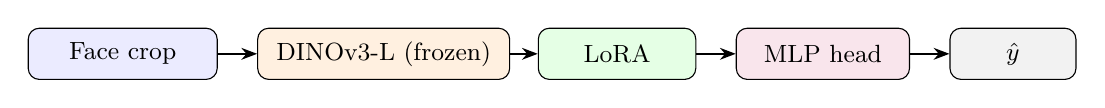
\begin{tikzpicture}[
  box/.style={draw, rounded corners, minimum height=0.65cm, font=\small},
  arr/.style={-{Stealth[length=2mm]}, thick}
]
  \node[box, fill=blue!8, minimum width=2.4cm] (img) {Face crop};
  \node[box, fill=orange!12, minimum width=3.2cm, right=0.5cm of img] (bb) {DINOv3-L (frozen)};
  \node[box, fill=green!10, minimum width=2.0cm, right=0.35cm of bb] (lora) {LoRA};
  \node[box, fill=purple!10, minimum width=2.2cm, right=0.5cm of lora] (head) {MLP head};
  \node[box, fill=gray!10, minimum width=1.6cm, right=0.5cm of head] (out) {$\hat{y}$};
  \draw[arr] (img) -- (bb);
  \draw[arr] (bb) -- (lora);
  \draw[arr] (lora) -- (head);
  \draw[arr] (head) -- (out);
\end{tikzpicture}
\caption{Submitted pipeline: frozen DINOv3-L backbone with LoRA adapters and a lightweight MLP head.}
\label{fig:arch}
\end{figure}

\paragraph{Training.}
AdamW ($\mathrm{lr}{=}5{\times}10^{-4}$, weight decay $10^{-4}$), cosine schedule with 1-epoch warmup, gradient clipping at 1.0; 15 epochs, batch size 64 on one RTX~3090 ($\sim$6\,h).
The best checkpoint (epoch~8) is submitted.

\section*{Results}
\begin{table}[h]
\centering
\caption{Best validation scores across explored models (lower is better).}
\label{tab:baselines}
\small
\begin{tabular}{@{}lcccc@{}}
\toprule
\textbf{Model} & \textbf{Score} & $\mathrm{Err}_F$ & $\mathrm{Err}_M$ & \textbf{Ep.} \\
\midrule
\multicolumn{5}{@{}l}{\textit{Phase 1 --- CNN/ViT baselines}} \\
Swin-T & 0.001090 & 0.000481 & 0.000887 & 14 \\
ConvNeXt-Tiny & 0.001112 & 0.000671 & 0.000965 & 3 \\
ViT-B/16 & 0.001162 & 0.000563 & 0.000962 & 8 \\
ResNet-50 & 0.001221 & 0.000536 & 0.000992 & 11 \\
EfficientViT-B1 & 0.001285 & 0.000660 & 0.001076 & 8 \\
DINOv2-Small & 0.001469 & 0.000693 & 0.001210 & 18 \\
\midrule
\multicolumn{5}{@{}l}{\textit{Phase 2 --- balanced-gender batching}} \\
Swin-T (balanced) & 0.001150 & 0.000547 & 0.000949 & 10 \\
\midrule
\multicolumn{5}{@{}l}{\textit{Phase 3 --- DINOv3 (submitted model in bold)}} \\
\textbf{DINOv3-L + LoRA} & \textbf{0.001059} & \textbf{0.000567} & \textbf{0.000895} & 8 \\
DINOv3-L + LoRA (balanced) & 0.001129 & 0.000525 & 0.000928 & 14 \\
\bottomrule
\end{tabular}
\end{table}

\begin{figure}[t]
\centering
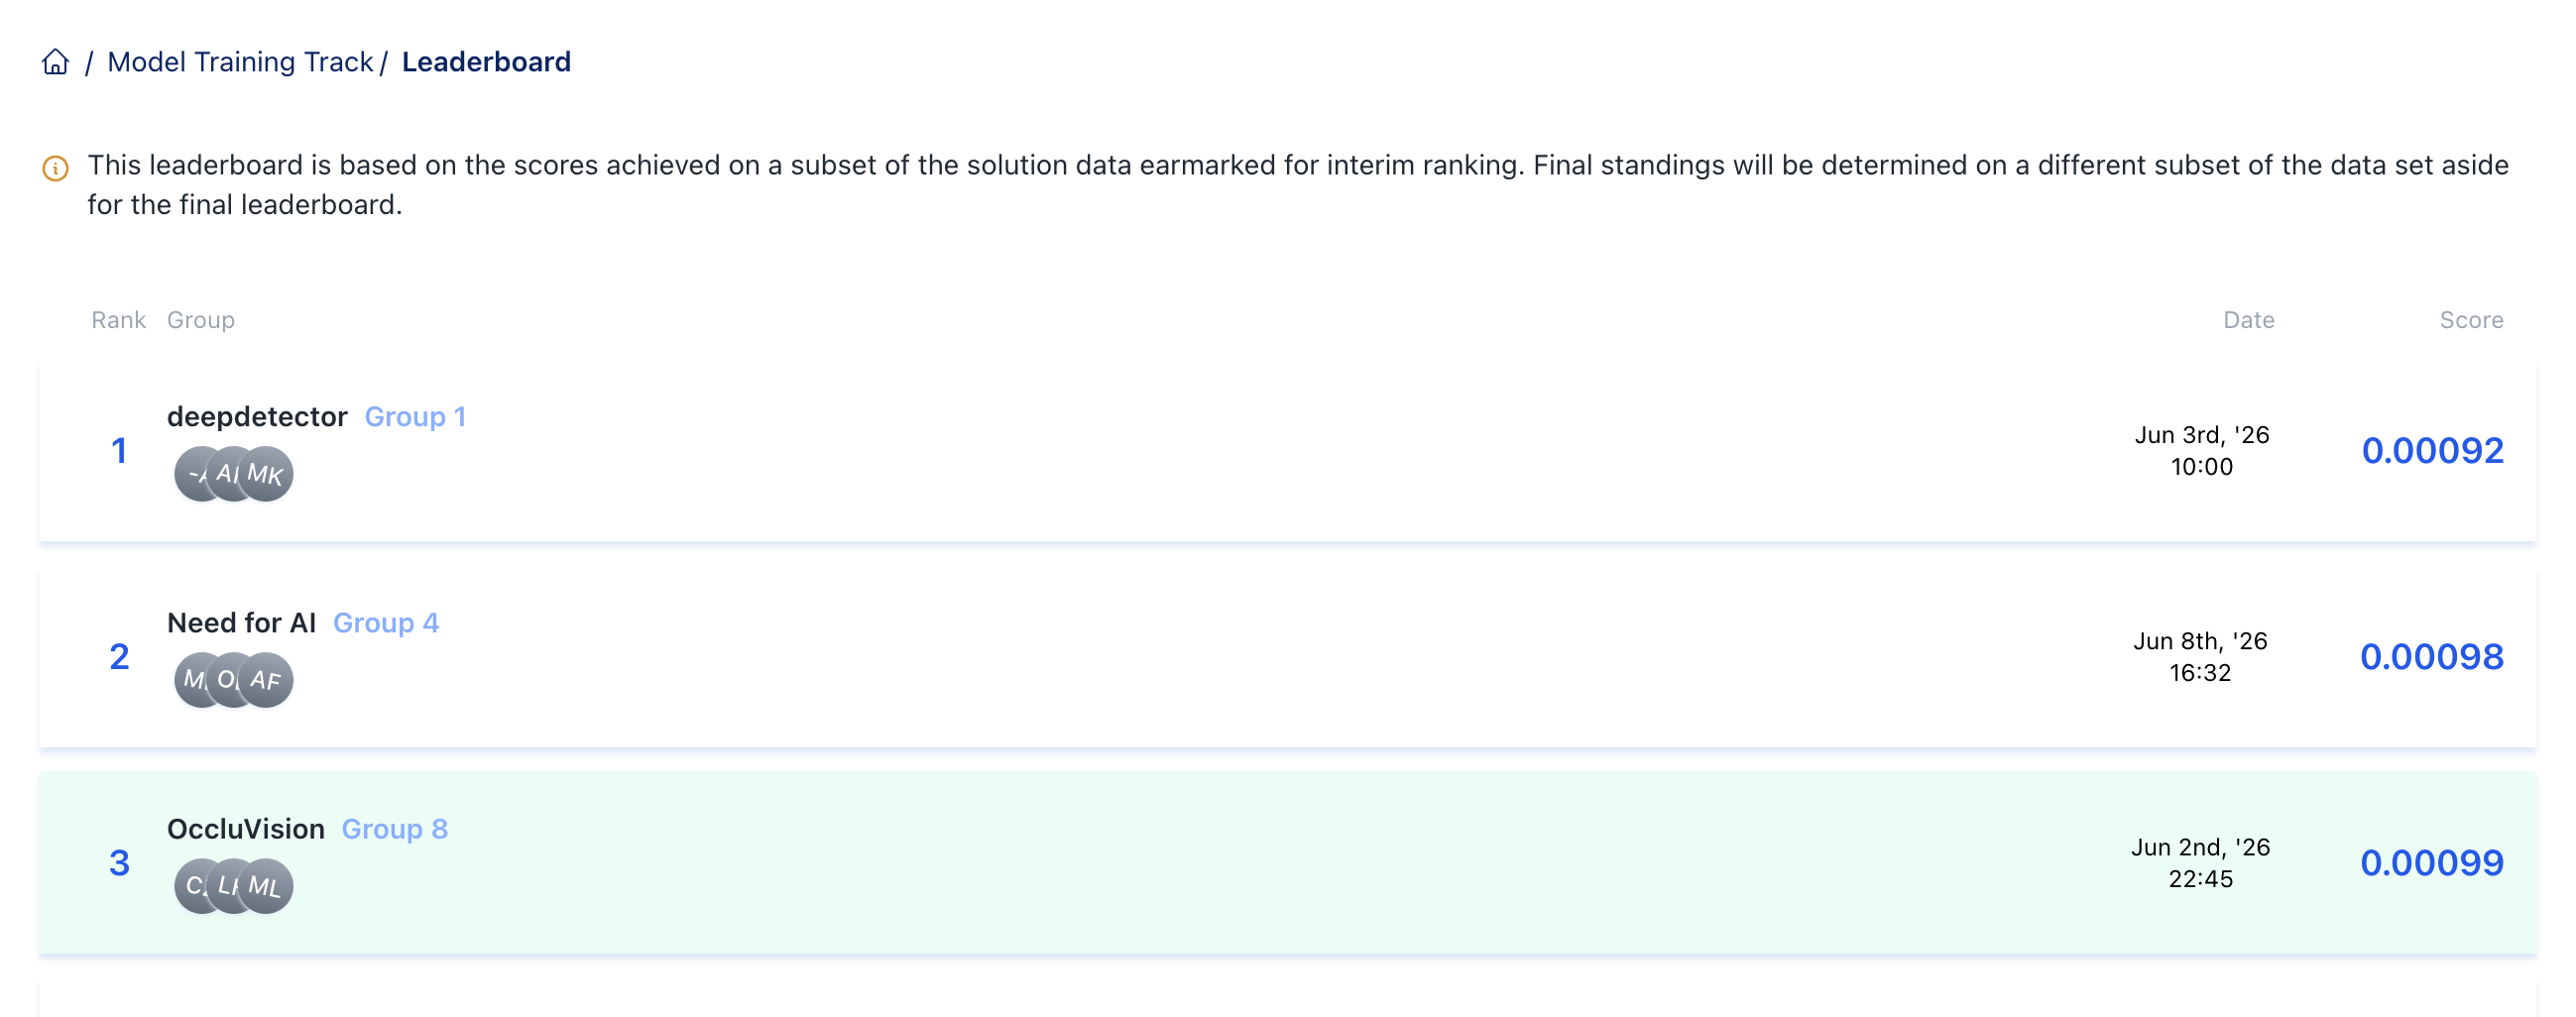
\includegraphics[width=0.48\linewidth]{figures/leaderboard.png}
\caption{Interim leaderboard (final ranking uses a different test subset).}
\label{fig:lb}
\end{figure}

\section*{Limitations \& Outlook}
\paragraph{Limitations.}
\begin{itemize}
  \item \textbf{Compute:} Limited training budget---all experiments were capped at 20 epochs, which may leave performance on the table.
  \item \textbf{Hyper-parameters:} LoRA rank, learning rate, batch size, and epoch count all affect the fairness--accuracy trade-off; we did not run a full grid search.
  \item \textbf{Gender gap:} Despite the metric penalty, male error remains higher than female error on validation.
\end{itemize}
\paragraph{Future work.}
\begin{itemize}
  \item \textbf{Close the gender gap:} combine LoRA fine-tuning with balanced-gender batching (which lowered $\mathrm{Err}_F$ in isolation) and tune the loss to better match the $|{\mathrm{Err}_F - \mathrm{Err}_M}|$ penalty.
  \item \textbf{Ensemble:} average or stack predictions from DINOv3-L + LoRA with strong CNN/ViT baselines (e.g.\ Swin-T) to exploit complementary errors.
  \item \textbf{Final retraining:} once the best configuration is fixed, retrain on train\,+\,val and submit the resulting checkpoint.
\end{itemize}

\end{document}
